\documentclass[10pt,a4paper]{article}
\usepackage[margin=2.2cm]{geometry}
\usepackage[T1]{fontenc}
\usepackage[utf8]{inputenc}
\usepackage{newpxtext,newpxmath}
\usepackage{microtype}
\usepackage{graphicx}
\usepackage{booktabs}
\usepackage{array}
\usepackage{siunitx}
\usepackage{amsmath}
\usepackage[round,sort]{natbib}
\setcitestyle{aysep={},citesep={,}}
\usepackage[font=small,labelfont=bf,skip=4pt]{caption}
\usepackage{enumitem}
\usepackage{xcolor}
\usepackage{tikz}
\usetikzlibrary{arrows.meta,positioning,calc,shapes.misc}
\PassOptionsToPackage{hyphens}{url}
\usepackage[colorlinks,linkcolor=black,citecolor=black!70,urlcolor=black!70]{hyperref}
\usepackage{url}
\urlstyle{same}
\setlength{\parskip}{2pt}\setlength{\bibsep}{2.5pt}\renewcommand{\bibfont}{\small\raggedright}
\setlength{\parindent}{1.2em}
\sisetup{range-phrase = { to }, range-units = single, per-mode = symbol}
\newcommand{\ugm}{\si{\micro\gram\per\cubic\metre}}
\newcommand{\load}{M\,person\,\ugm\,h/day}
\newcommand{\eps}{\varepsilon}
\newcommand{\Win}{W_{\mathrm{in}}}
\setlist{nosep, leftmargin=1.4em}
\graphicspath{{figures/}}
\definecolor{b1}{HTML}{2a78d6}\definecolor{b2}{HTML}{eb6834}\definecolor{b3}{HTML}{1baf7a}\definecolor{b4}{HTML}{4a3aa7}\definecolor{ink2}{HTML}{52514e}\definecolor{grid}{HTML}{e6e5e0}
\tikzset{sbox/.style={draw=ink2, rounded corners=2pt, line width=0.5pt, align=center, font=\small, inner sep=5pt, minimum height=1.05cm, text width=3.15cm},
         meth/.style={font=\scriptsize\itshape, text=ink2, align=center, text width=3.3cm},
         cnt/.style={font=\scriptsize, align=center, text width=3.3cm},
         arr/.style={-{Stealth[length=5pt]}, line width=0.6pt, ink2}}

\title{\Large\bfseries From a cited implication graph to one buildable intervention:\\ choosing an air-pollution problem and its solution for Abu Dhabi by network decomposition, exposure load and multi-criteria screening}
\author{Karthik Nambiar \and Sumedh Nitin Jamsandekar \and Ti\kern0pt ju\\[4pt]
\normalsize IIT Delhi Abu Dhabi, AGRL130 Innovation, Entrepreneurship and Sustainability, week 3}
\date{\normalsize 21 September 2026}

\begin{document}
\maketitle

\begin{abstract}
\noindent Picking one air-pollution problem in Abu Dhabi and one intervention a student group can pilot in a semester is a selection problem, and we treat it as one. An implication graph of the city's air-pollution system was built in the WHO DPSEEA frame from 418 cited edge rows (160 nodes, 337 distinct edges, 238 source lines with 173 distinct DOIs, every source fetched at origin). A network decomposition inspired by Simon and Ando's near-decomposability, a leakage ratio on blocks found by directed modularity, tested under 200 weight perturbations, five resolutions, two other partition algorithms, 50 seeds, random removal of lower-tier evidence and leave-one-source-out, returns four candidate problem modules. An exposure-load criterion (people \(\times\) hours \(\times\) PM\(_{2.5}\) increment) ranks them with every input sourced: construction workers \num{16.9} million person\,\ugm\,h per day, near-road residents and riders \num{7.0}, the child commute \num{4.5}, the school gate \num{0.68}. Morphological generation over the modules' cited edges produced 332 interventions in four mechanism classes. Four conjunctive gates and an eleven-criterion weighted-sum rubric screened them, stochastic multicriteria acceptability analysis (10,000 draws) measured the ranking's dependence on the weights and, separately, on the scores, and a failure-mode analysis in the premortem form fixed the design specification. The intervention that meets it, Clean Cabin, is a measurement-driven service: find which school buses pollute their own cabin, identify why, apply the smallest compatible source-side repair, and verify it with the same paired sensors. It scores 79 of 90, holds rank 1 in 86\,\% of draws over the weights with no weight information at all and under every leave-one-criterion-out ranking, and rank 1 in 48\,\% and top 3 in 72\,\% of draws in which every score is also moved by one level. The self-pollution physics and the source-side repairs carry twenty years of measured evidence, none of it found applied to Abu Dhabi's school buses, which carried 237,111 pupils on 8,568 buses in 2024 and more than 279,000 on more than 10,000 in 2026.
\end{abstract}

\section{The question and the method}
The week 3 brief asks for four things: restate the need, show every solution explored, state the filters used including our own, and apply them to one final solution. That is a two-level selection: a problem from a system in which everything touches everything, then an intervention from the many that could act on it. Each level is answered here by a named, published method with a reproducible artefact (Figure~\ref{fig:pipeline}). The literature harvest that produced the edge table was scripted lane by lane, every candidate source fetched at its origin before its row was accepted, and every row carries its citation, identifier and the sentence it rests on. The graph, the decomposition, the exposure arithmetic, the intervention inventory, every gate decision and every score are the authors' work, and the files that reproduce every figure are listed in Appendix~\ref{app:repro}.

\begin{figure}[t]\centering
\begin{tikzpicture}[node distance=0.55cm and 0.45cm]
\node[sbox] (g) {\textbf{1 Evidence graph}\\160 nodes, 418 cited rows};
\node[sbox, right=of g] (d) {\textbf{2 Decomposition}\\9 blocks, 4 separable};
\node[sbox, right=of d] (l) {\textbf{3 Exposure load}\\4 modules ranked};
\node[sbox, right=of l] (p) {\textbf{4 Problems}\\5 need statements};
\node[sbox, below=of p] (s) {\textbf{5 Screening}\\332 \(\to\) 232 \(\to\) 1};
\node[sbox, left=of s] (r) {\textbf{6 Failure modes}\\29 modes, 5 fatal};
\node[sbox, left=of r, draw=b3, line width=0.9pt] (c) {\textbf{7 Clean Cabin}\\79 of 90, diagnose, repair, verify};
\draw[arr] (g) -- (d); \draw[arr] (d) -- (l); \draw[arr] (l) -- (p); \draw[arr] (p) -- (s); \draw[arr] (s) -- (r); \draw[arr] (r) -- (c);
\node[meth, above=0.08cm of g] {DPSEEA frame, ordinal weights, evidence tiers};
\node[meth, above=0.08cm of d] {leakage ratio on directed-modularity blocks, after Simon and Ando};
\node[meth, above=0.08cm of l] {Ott's integrated exposure over microenvironments};
\node[meth, above=0.08cm of p] {one microenvironment per problem, boundaries stated};
\node[meth, below=0.08cm of s] {morphological generation, gates, weighted sum, SMAA over weights and scores};
\node[meth, below=0.08cm of r] {premortem structured as FMEA};
\node[meth, below=0.08cm of c] {paired cabin and roof measurement, per-bus diagnosis and verification};
\end{tikzpicture}
\caption{The seven steps and their counts. Each box is a section below, each method line names the published method the step instantiates.}\label{fig:pipeline}\end{figure}

\section{Step 1: the evidence graph}\label{sec:graph}
Nodes follow the DPSEEA chain the WHO adopted for environmental-health indicators \citep{Corvalan1999}: a \emph{driving force} creates a \emph{pressure} (an emission), which changes a \emph{state} (a concentration at a place), to which people are \emph{exposed} for a time, with an \emph{effect}, and on which an \emph{action} acts. Each node is a defined quantity with a unit where one exists and a scope. The list has 26 driving forces, 33 pressures, 34 states, 19 exposures, 20 effects and 28 actions. An edge is a directed influence documented by a fetched source and carries a sign, a weight, a tier, a scope, the citation, an identifier and the sentence it rests on (Table~\ref{tab:rules}). Where an Abu Dhabi or UAE source-apportionment number exists the measured share is recorded beside the ordinal weight (29 of 418 rows). Duplicate rows for a node pair are kept as separate evidence lines and the pair takes the maximum weight.

\begin{table}[t]\centering\small
\caption{Edge rules, fixed before the harvest.}\label{tab:rules}
\begin{tabular}{@{}clp{10.6cm}@{}}\toprule
field & level & rule\\ \midrule
weight & 3 & the source identifies the origin as the dominant or primary driver of the destination, or a quantified contribution of 30\,\% or more\\
 & 2 & a substantial documented contribution, 10 to 30\,\%, or ``major but not primary''\\
 & 1 & documented and minor, under 10\,\%, or only the mechanism is shown\\
tier & 1 to 4 & systematic review or WHO-grade synthesis, primary measured study, modelling study or official statistic or technical report, grey literature\\
scope & & Abu Dhabi, UAE, Gulf or global, with cross-boundary sources (regional dust, transboundary PM) kept as source nodes\\
\bottomrule\end{tabular}\end{table}

The harvest ran in eight lanes, one per layer pair or theme, in two passes, the second adding nodes for every problem raised in class so that each candidate has comparable detail (Figure~\ref{fig:coverage}). A validator rejected any row without an identifier or a fetch flag. The result is 418 edge rows, 337 distinct edges, 238 source lines with 173 distinct DOIs among them, all fetched on 20 September 2026: by weight 97, 179 and 142 rows at levels 1, 2 and 3, by tier 95, 217, 78 and 28, by scope 243 global, 64 Gulf, 38 UAE and 73 Abu Dhabi. The total internal weight is 720 and five nodes are isolated. Figure~\ref{fig:graph} shows the whole graph.

\begin{figure}[t]\centering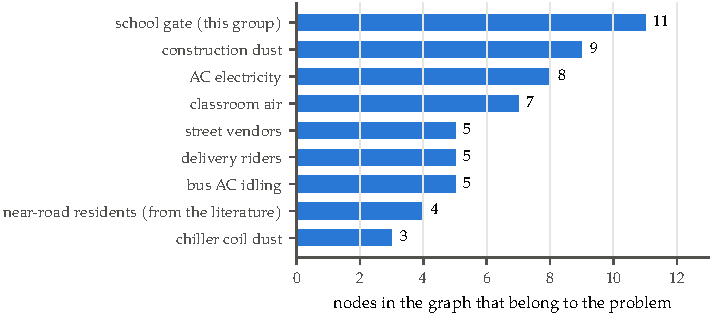
\includegraphics[width=0.62\textwidth]{fig4-coverage}
\caption{Coverage: nodes in the graph that belong to each problem raised in class (fixed node sets, Appendix~\ref{app:repro}). Every candidate problem is represented with three to eleven dedicated nodes, the condition under which a decomposition can be compared across them.}\label{fig:coverage}\end{figure}

\begin{figure}[p]\centering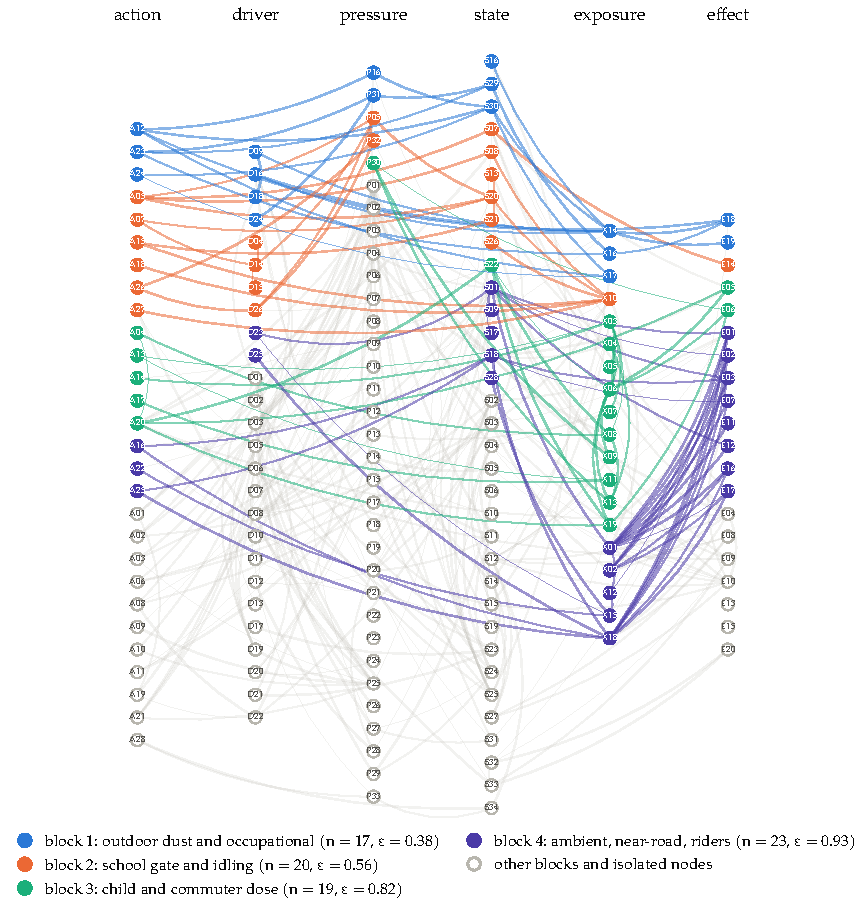
\includegraphics[width=\textwidth]{fig1-graph}
\caption{The 160-node implication graph by DPSEEA layer, every edge a cited influence (line weight follows the ordinal weight). Nodes and internal edges of the four separable blocks of Section~\ref{sec:decomp} are coloured: construction sites, their workers and neighbours and the street vendors (blue), the school gate and vehicle idling (orange), the child's time-activity and dose (green), ambient PM with near-road residents, delivery riders and the city's health burden (violet).}\label{fig:graph}\end{figure}

\section{Step 2: a network decomposition, inspired by near-decomposability, finds the problem modules}\label{sec:decomp}
\citet{AndoSimon1961} showed that a dynamical system whose interaction matrix is block-diagonal apart from small off-block terms behaves, in the short run, as independent subsystems, and \citet{Simon1962} argued that this is what makes complex systems tractable. We borrow the idea, not the theorem. The graph's weights are ordinal, literature-derived statements of influence, not a physical interaction matrix, so what the decomposition below establishes is that a block's concepts are more densely and more strongly connected to one another in the evidence than to the rest, and what it does not establish is that an intervention inside the block has contained real-world consequences. The blocks are therefore a menu of candidates, ranked by a criterion stated outside the graph (Section~\ref{sec:load}) and tested by a pilot (Section~\ref{sec:cabin}). A candidate problem is a block whose internal coupling dominates its coupling to the rest. For a node set \(S\) with weights \(w_{ij}\in\{1,2,3\}\),
\begin{equation}
\Win(S)=\sum_{i,j\in S} w_{ij},\qquad
\eps_{\mathrm{out}}=\frac{\sum_{i\in S,\,j\notin S} w_{ij}}{\Win},\qquad
\eps_{\mathrm{in}}=\frac{\sum_{i\notin S,\,j\in S} w_{ij}}{\Win},\qquad
\eps_{\mathrm{sym}}=\eps_{\mathrm{out}}+\eps_{\mathrm{in}},
\end{equation}
and \(\eps_{\mathrm{transfer}}\) is the part of \(\eps_{\mathrm{out}}\) that lands on driver, pressure or state nodes, the load that acting inside \(S\) moves elsewhere. A block \emph{qualifies} when it holds an action node and an exposure or effect node, and is \emph{separable} when \(\eps_{\mathrm{sym}}<1\). An anchor test with two planted dense blocks joined by one weak edge returns a planted block with leakage equal to that edge over \(\Win\), which fixes the scale. Blocks come from directed modularity \citep{LeichtNewman2008} maximised by Louvain \citep{Blondel2008} with the directed gain of \citet{DuguePerez2015}, resolution 1.0, seed 0.

\begin{table}[t]\centering\small
\caption{The nine blocks of two or more nodes. A block qualifies with an action and an outcome inside it.}\label{tab:blocks}
\footnotesize\begin{tabular}{@{}clcrrrrrr@{}}\toprule
rank & block & qualifies & \(n\) & \(\Win\) & \(\eps_{\mathrm{sym}}\) & \(\eps_{\mathrm{out}}\) & \(\eps_{\mathrm{in}}\) & \(\eps_{\mathrm{transfer}}\)\\ \midrule
1 & outdoor dust and occupational (construction, vendors) & yes & 17 & 56 & 0.375 & 0.250 & 0.125 & 0.214\\
2 & school gate and idling & yes & 20 & 63 & 0.556 & 0.365 & 0.190 & 0.143\\
3 & child and commuter time-activity and dose & yes & 19 & 62 & 0.823 & 0.290 & 0.532 & 0.081\\
4 & ambient PM, near-road residents, riders, health burden & yes & 23 & 91 & 0.934 & 0.363 & 0.571 & 0.066\\
5 & dust, PM\(_{10}\), chiller-coil fouling & yes & 16 & 60 & 1.350 & 0.633 & 0.717 & 0.350\\
6 & two-node fragment & no & 2 & 1 & 0.000 & 0.000 & 0.000 & 0.000\\
7 & energy, cooling and industry & no & 26 & 89 & 0.258 & 0.124 & 0.135 & 0.101\\
8 & traffic emissions, NO\(_x\), ozone, fleet levers & no & 28 & 104 & 0.548 & 0.423 & 0.125 & 0.298\\
9 & classroom CO\(_2\), ventilation, cognition, absenteeism & no & 4 & 12 & 0.917 & 0.083 & 0.833 & 0.000\\
\bottomrule\end{tabular}\end{table}

\begin{figure}[t]\centering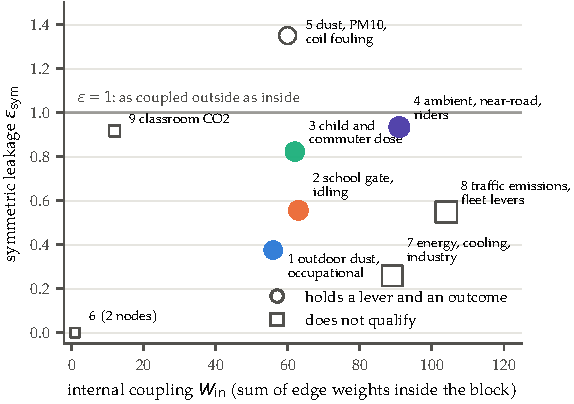
\includegraphics[width=0.62\textwidth]{fig2-leakage}
\caption{Symmetric leakage against internal coupling. Circles qualify, squares do not, marker area follows node count. Everything below \(\eps=1\) is more coupled inside than across its boundary. The four coloured blocks are the menu.}\label{fig:leak}\end{figure}

\textbf{Partition.} \(Q=0.604\), nine blocks of two or more nodes and five isolated nodes (Table~\ref{tab:blocks}, Figure~\ref{fig:leak}). Four qualify and are separable: (1) outdoor dust and occupational exposure, construction sites with their workers and neighbours, street vendors and migrant labour, 17 nodes, \(\eps_{\mathrm{sym}}=0.375\), and the lowest dependence on outside inputs (\(\eps_{\mathrm{in}}=0.125\)), because dust at a fenceline or smoke at a stall is made locally. (2) The school gate and idling, 20 nodes, \num{0.556}, with six actions, the most of any block. (3) Child and commuter time-activity and dose, 19 nodes, \num{0.823}. (4) Ambient PM with near-road residents and delivery riders and the city's health burden, 23 nodes, \num{0.934}. The energy and traffic blocks are the tightest subsystems in the graph but hold no exposure or effect node, and the classroom CO\(_2\) chain has no action inside it. Blocks 2 and 3 are the two halves of the school system, sources and levers on one side, the child's dose and effects on the other, joined by gate concentration to child time at the gate (S20 to X04) and classroom exposure to child dose (X10 to X06).

\textbf{Stability} (Figure~\ref{fig:perturb}). \emph{Resolution:} the school block is identical at 0.8 and 1.0 and reappears at Jaccard 0.70 \citep{Jaccard1912} at 1.2 and 1.5, the near-road block is identical at 1.0 and 1.2 and reappears at 0.87 at 1.5, and at 0.6 block 1 is unchanged while blocks 2 and 3 merge. \emph{Algorithm:} Leiden \citep{Traag2019} returns the school block at Jaccard 0.85 and Clauset-Newman-Moore greedy modularity \citep{Clauset2004} at 0.95. \emph{Weights:} with every ordinal weight bumped one level at random 200 times, the school block reappears at Jaccard 0.6 or better in 66\,\% of trials (mean 0.668), the other three in 29 to 30\,\% (mean 0.53 to 0.54). The rank order is less stable than the membership: block 1 leaks least in 40\,\% of trials, block 2 in 10\,\%, and the five-node street-vendor chain, a fragment of block 1, in 34\,\%. \emph{Seeds:} 50 Louvain seeds return the blocks at mean Jaccard 0.63 to 0.78.

\textbf{Inclusion} (Table~\ref{tab:dropout}). Re-weighting the evidence does not test what the largest uncertainty is, which rows made it into the graph at all. Three tests do. Dropping 10\,\% of the tier 3 and 4 rows at random, 200 times, returns the school block at Jaccard 0.6 or better in 97\,\% of trials, the construction and commute blocks in 83 and 73\,\%, the near-road block in 57\,\%, and 20\,\% dropout changes those figures by at most eight points. Leaving out one of the 207 cited sources at a time returns the school, construction and commute blocks at 0.6 or better in 97, 99 and 92\,\% of the 207 rebuilds, the near-road block in 9\,\% (mean 0.56, worst case 0.44 when the HEI traffic review is removed). Rebuilding on tier 1 and 2 evidence alone, 312 of the 418 rows, recovers the four blocks at Jaccard 0.40 to 0.58 only: the tier 3 and 4 rows are part of what holds the blocks together. The menu is stable to small losses of evidence and to any single source, and the near-road block is the one whose membership depends most on which studies were read.

\begin{table}[t]\centering\small
\caption{Inclusion robustness: Jaccard similarity between each baseline block and its best match after the evidence is thinned. Share of rebuilds at 0.6 or better, mean in parentheses.}\label{tab:dropout}
\begin{tabular}{@{}lcccc@{}}\toprule
test & 1 construction & 2 school gate & 3 commute & 4 near-road\\ \midrule
drop 10\,\% of tier 3 and 4 rows, 200 trials & 83\,\% (0.62) & 97\,\% (0.72) & 73\,\% (0.76) & 57\,\% (0.66)\\
drop 20\,\% of tier 3 and 4 rows, 200 trials & 75\,\% (0.64) & 97\,\% (0.73) & 73\,\% (0.74) & 56\,\% (0.64)\\
leave one source out, 207 rebuilds & 99\,\% (0.78) & 97\,\% (0.67) & 92\,\% (0.85) & 9\,\% (0.56)\\
tier 1 and 2 rows only, one rebuild & 0.55 & 0.50 & 0.40 & 0.58\\
\bottomrule\end{tabular}\end{table}

\begin{figure}[t]\centering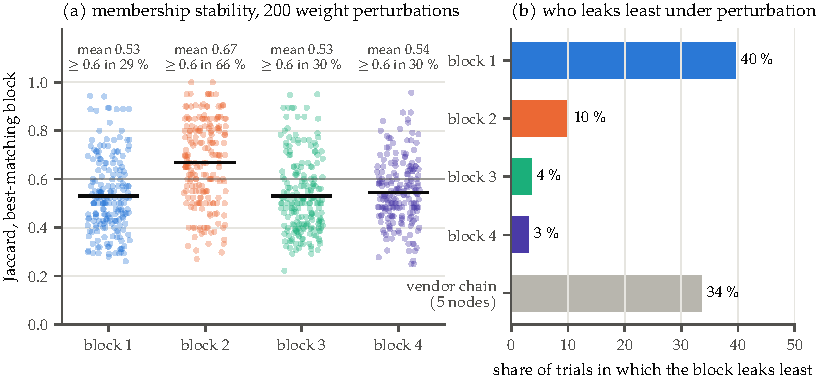
\includegraphics[width=0.92\textwidth]{fig3-perturbation}
\caption{Stability under 200 random one-level perturbations of every edge weight. (a) Jaccard similarity between each block and its best-matching block in the perturbed partition, one dot per trial, bar at the mean. (b) Share of trials in which each block is the lowest-leakage qualifying block.}\label{fig:perturb}\end{figure}

\textbf{What the step delivers.} A menu of four candidate problems with a lever and an outcome inside each, and a measured stability for it under re-weighting and under thinning of the evidence. Leakage is a ratio, so a small closed chain scores well however little it matters, which is why the vendor chain wins a third of the perturbed reruns. Ranking the menu needs a criterion stated outside the graph, which is step 3.

\section{Step 3: exposure load ranks the menu}\label{sec:load}
\citet{Ott1982} defined a person's exposure as the integral of concentration over time in contact with it, and \citet{Duan1982} showed it can be computed piecewise over microenvironments. Summed over the people in a microenvironment,
\begin{equation}
L=N\times h\times\Delta C,
\end{equation}
with \(N\) the people in it, \(h\) their hours per day there and \(\Delta C\) the PM\(_{2.5}\) increment the block's own sources add, in person\,\ugm\,h per day, reported in millions. PM\(_{2.5}\) is the one pollutant every block has a fetched increment for. The metric measures where a block's own pollution meets the most breathing. It does not weight susceptibility or toxicity per microgram (Section~\ref{sec:limits}). Intake fraction \citep{Bennett2002} would need an emission rate per source, which no block has for Abu Dhabi.

\begin{table}[t]\centering\footnotesize
\caption{The exposure-load terms, \(L=N\times h\times\Delta C/10^6\) in \load. Ranges follow the stated low and high values of each assumed input. Rows in italics could not be computed for want of a count. \(^{\dagger}\)\,\(N=2.8\,\mathrm{M}\times f\) with \(f=0.3\) (0.2 to 0.5) the unsourced fraction of the Abu Dhabi Region living within 300 m of an arterial, and \(\Delta C=0.85\) (0.6 to 1.1) \(\times\) an indoor-to-outdoor ratio of 0.5 (0.4 to 0.6). The riders' high bound uses the roadway concentration of 13. The gate's high bound uses the measured 4.11.}\label{tab:load}
\begin{tabular}{@{}clrccl@{}}\toprule
block & microenvironment & \(N\) & \(h\) (h/day) & \(\Delta C\) (\ugm) & \(L\)\\ \midrule
1 & construction workers on site & 324,879 & 8 & 6.5 (5 to 8) & \textbf{16.9} (13.0 to 20.8)\\
1 & \emph{site-neighbour residents} & \emph{no count} & 16 & \emph{none extracted at 100 m} & \emph{not computed}\\
1 & \emph{vendors at charcoal or gas stalls} & \emph{no count} & 10 & 152 & \emph{1.5 per 1,000 vendors}\\
2 & pupils in the gate zone & 396,230 & 0.5 (0.25 to 0.75) & 3.45 (3.45 to 4.11) & \textbf{0.68} (0.34 to 1.22)\\
3 & pupils on school buses & 237,111 & 1.33 & 13 & 4.11\\
3 & pupils driven by car & 115,676 & 0.67 & 3 & 0.23\\
3 & pupils walking & 43,443 & 0.5 & 6 & 0.13\\
3 & total & & & & \textbf{4.47} (4.3 to 4.7)\\
4 & delivery riders on the road & 26,186 & 8 (6 to 10) & 6 (6 to 13) & 1.26 (0.94 to 3.40)\\
4 & near-road residents at home\(^{\dagger}\) & 840,000 & 16 & 0.43 & 5.7 (2.2 to 14.8)\\
4 & total & & & & \textbf{7.0} (3.1 to 18.2)\\
\bottomrule\end{tabular}\end{table}

\textbf{Inputs} (Table~\ref{tab:load}). Populations are Abu Dhabi statistics: 396,230 pupils in 2022 \citep{ADCCI2024}, 2,762,715 employed persons at 30 September 2024 \citep{SCAD2024labour} of whom 14.1\,\% work in construction \citep{SCAD2020yearbook}, so \(2{,}762{,}715\times0.141=389{,}543\), of whom 83.4\,\% work outdoors after \citet{AlHurini2024} (331 of 397 labour-camp workers outdoors over two hours a day), so \(389{,}543\times0.834=324{,}879\). School transport carries 237,111 pupils on 8,568 buses run by 206 operators at 672 schools and nurseries \citep{ADM2024buses}, 59.8\,\% of the roll, with the car-to-walk split of the remainder from \citet{Badri2012}. Delivery riders are the 26,186 commercial motorcycles \citep{ADM2024moto}. The 2024 population is 4,135,985 with 68.2\,\% in the Abu Dhabi Region \citep{SCAD2025pop}. Increments come from measured studies elsewhere. Bus cabin: in-cabin PM\(_{2.5}\) \(20\pm18\) against ambient \(7\pm5\) and roadway \(13\pm12\)\,\ugm\ over 597 trips on 188 buses, mean trip 40 minutes \citep{Adar2015}. School gate: a mean drop-off increment of \num{3.45} across 86 schools \citep{AdamsRequia2017}, \num{4.11} measured at the most-bused of four schools \citep{Ryan2013}. Construction: fine-fraction increment of 5 to 8 (PM\(_{10}\) about 110 to 125) from a demolition site's fixed and mobile measurements against background \citep{Azarmi2016}, diesel elemental carbon 3.4 against 0.9 on site \citep{Ferree2024}. Near-road: 31 US near-road PM\(_{2.5}\) monitors run 6 to 10\,\% above average, 0.6 to 1.1\,\ugm\ \citep{Seagram2019}, the zone of influence for PM mass 100 to 400 m \citep{ZhouLevy2007}, and many studies find no PM-mass gradient at all \citep{Karner2010}, so this is an upper end. Indoor-to-outdoor 0.4 to 0.6 in sealed Gulf homes \citep{Yuan2020}, motorcycle at four times a car \citep{Patel2016}, time at home from the US activity survey \citep{Klepeis2001}, the charcoal-cart microenvironment of 196\,\ugm\ from New York \citep{Nahar2020}.

\begin{figure}[t]\centering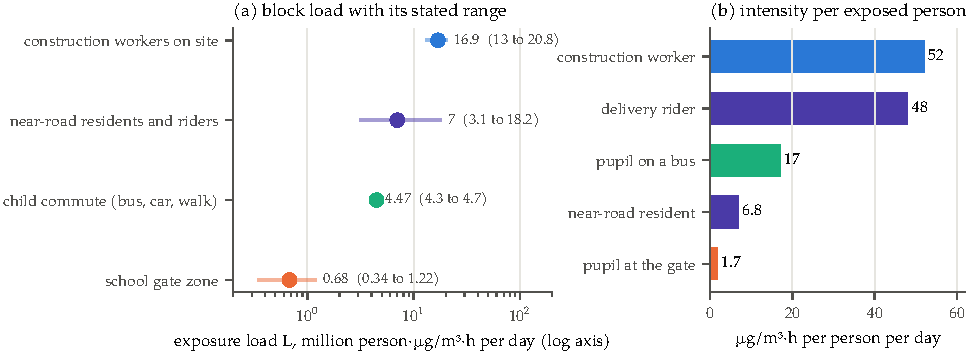
\includegraphics[width=0.92\textwidth]{fig5-loads}
\caption{(a) Exposure load per block on a log axis with the range implied by the stated low and high inputs. (b) The same arithmetic per exposed person.}\label{fig:load}\end{figure}

\textbf{Result} (Figure~\ref{fig:load}). Construction workers \num{16.9}\,\load\ (13.0 to 20.8), near-road residents and riders \num{7.0} (3.1 to 18.2), the child commute \num{4.47} (4.3 to 4.7) of which the bus term alone is \num{4.11}, the school gate \num{0.68} (0.34 to 1.22). Per person per day: a construction worker 52\,\ugm\,h, a delivery rider 48, a bus pupil 17, a near-road resident 6.8, a pupil at the gate 1.7. In PM\(_{10}\) the construction row is 299 M against an Abu Dhabi Region ambient of 114.6\,\ugm\ \citep{SCAD2024air}, so a site roughly doubles what a worker breathes. By impact the menu picks outdoor construction labour, then near-road residents. What a three-student group can reach, change and measure within a semester is a set of criteria of its own, and step 4 states them and applies them to every candidate intervention rather than to the problem in the abstract.

\section{Step 4: generating and screening the interventions}\label{sec:funnel}
\textbf{Five problems.} Block 1 holds two receptor groups with different sources and is split, so that each need statement has one microenvironment (Table~\ref{tab:problems}).

\begin{table}[t]\centering\small
\caption{The five problems, each with its inclusion boundary, its exclusion boundary and its load.}\label{tab:problems}
\footnotesize\begin{tabular}{@{}lp{4.4cm}p{3.4cm}r@{}}\toprule
problem & in & out & \(L\)\\ \midrule
P1 construction workers and site neighbours & the dust source, the fenceline, the two exposed groups & vendors, traffic, dust storms & 16.9\\
P2 street food vendors & fuel, stall, concentration, vendor & customers, kitchens, traffic & no count\\
P3 school gate and idling & car and bus idling, gate concentration, infiltration, classroom & the commute, home, ambient dust & 0.68\\
P4 child commute and daily dose & time-activity, in-vehicle air, breathing rate, peaks, lung and cognition & the gate, the sources & 4.47\\
P5 near-road residents and delivery riders & the near-road gradient, on-road air, the two groups, their outcomes & schools, sites, stalls, regional dust & 7.0\\
\bottomrule\end{tabular}\end{table}

\textbf{Generation by morphological analysis on the edges.} Every internal edge of a problem block is a documented mechanism and therefore a place to intervene. Following \citet{Zwicky1969} as formalised by \citet{Ritchey2006}, the generation space is the product of the block's internal edges and four mechanism classes, and every edge a student-scale intervention can act on was given at least one concrete intervention. The classes are the DPSEEA level at which the edge is cut: \emph{cut the source} (the pressure level), \emph{cut the path} (the state level), \emph{cut receptor time or intake} (the exposure level), and \emph{change the decision} (a rule, a price, information or enforcement, where the deeper leverage points of \citet{Meadows1999} sit). The four blocks hold 23, 25, 29 and 42 internal edges, block 1 serving P1 and P2. Interventions were written on 23, 24, 28 and 25 of them, 60, 50, 81, 71 and 70 rows for P1 to P5, 332 in all (Figure~\ref{fig:funnel}). The near-road block's seventeen edges without a row run from population exposure to health outcomes (mortality, cardiovascular and respiratory disease, birth outcomes, cancer), edges that carry no lever of their own. Each row carries its edge, so the mind map the brief asks for is the graph itself.

\textbf{Gates.} Four binary gates, the conjunctive form of a hard constraint \citep{BeltonStewart2002}, applied to all 332 before any scoring: \textbf{G1 reach}, the group can get to the user or the site this term, \textbf{G2 semester}, an effect can be produced and measured by December with instruments the group can borrow or buy, \textbf{G3 additive}, not already the standing rule or product in Abu Dhabi, \textbf{G4 no law change}. 232 pass. The near-road block loses most (28 of 70) because setbacks, zoning, fleet procurement and corridor measures need a regulator. Failed rows stay in the inventory with the gate that failed them.

\begin{figure}[t]\centering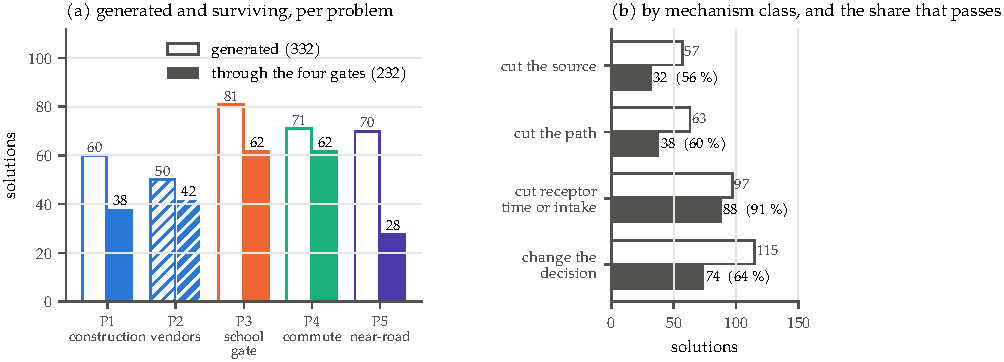
\includegraphics[width=0.92\textwidth]{fig6-funnel}
\caption{The funnel. (a) Interventions generated on each problem's edges and the number that pass the four gates (P2 hatched, it shares block 1 with P1). (b) The same by mechanism class. Receptor-side measures pass most often, they need fewer permissions, which is why the rubric carries a root-cause criterion.}\label{fig:funnel}\end{figure}

\textbf{Rubric.} Survivors are scored by a weighted-sum model \citep{Triantaphyllou2000}, the additive form appropriate when the criteria are preferentially independent \citep{KeeneyRaiffa1976}, on eleven criteria each scored 1 to 5 against written anchors with stated integer weights, maximum 90 (Table~\ref{tab:rubric}). Five criteria are the instructor's families. Six are ours: impact, anchored on the loads of step 3, measurability, time to effect, and the three that separate a cure from a shield, \emph{novelty}, \emph{cure} and \emph{transfer}, the last being the graph's own \(\eps_{\mathrm{transfer}}\) at the level of one intervention. The problem-level scores are child commute 70, vendors 69, construction 67, school gate 59, near-road 59. Among the 232 interventions the leaders are the per-bus cabin air service (79), a clean cooking zone pilot at one market (74), induction grills at stalls (73), LPG conversion (72), exhaust-leak inspection of every bus (71) and engine-off training for hired family drivers (71) (Figure~\ref{fig:scores}a).

\begin{table}[t]\centering\small
\caption{The eleven criteria, their weights and the anchors of the 5 and 1 levels.}\label{tab:rubric}
\begin{tabular}{@{}lcp{5.1cm}p{5.1cm}@{}}\toprule
criterion & weight & 5 & 1\\ \midrule
user & 1 & the exposed person asks for it & imposed with no felt benefit\\
feasibility & 2 & built or done with our resources this term & needs an organisation we are not\\
implementability & 2 & one person must say yes & a regulator plus an industry\\
usability & 1 & passive, no behaviour change & needs daily discipline\\
market and business & 1 & clear buyer, repeatable & none\\
impact & 3 & removes most of the block's load for everyone in the microenvironment & marginal\\
measurability & 2 & a before-and-after reading at one point & only a survey\\
time to effect & 1 & the day it is installed & years\\
novelty & 2 & nothing does this, a startup could own it & commodity product or standard rule\\
cure & 2 & removes the emission or the behaviour for everyone in the microenvironment & shields one receptor, source untouched\\
transfer & 1 & nothing moved elsewhere & burden moved to another group and to energy or waste\\
\bottomrule\end{tabular}\end{table}

\textbf{Criteria ablation} (Figure~\ref{fig:scores}b, Figure~\ref{fig:smaa}b). Removing novelty, cure and transfer leaves a rubric on which the cabin service and a bedroom air purifier tie at 58 of 65 and purifiers hold three of the top eight ranks. With the three criteria in, the purifiers fall to ranks 64 and beyond and the source-side rows lead by 15 points at the stated weights. The three criteria are what let the rubric measure what the brief asks for, a cure rather than a shield.

\begin{figure}[t]\centering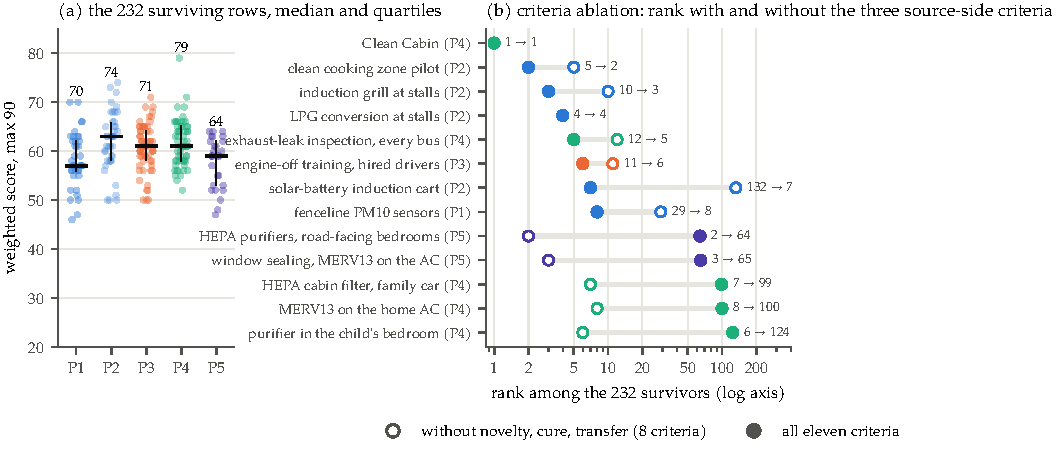
\includegraphics[width=\textwidth]{fig7-scores}
\caption{(a) Weighted scores of the 232 surviving interventions by problem, medians and quartiles, top score labelled. (b) Rank of the leading rows without (open) and with (filled) the three source-side criteria, on a log axis.}\label{fig:scores}\end{figure}

\textbf{Robustness to the weights.} Stochastic multicriteria acceptability analysis \citep{Lahdelma1998,LahdelmaSalminen2001} draws weight vectors from a distribution expressing what is known about the weights, ranks the alternatives under each draw, and reports the rank acceptability index \(b_i^r\), the share of draws in which alternative \(i\) holds rank \(r\) \citep{Butler1997,TervonenLahdelma2007}. Three distributions, 10,000 draws each, seed 0: \emph{centred}, a Dirichlet with concentration equal to the stated weights, \emph{\(\pm\)50\,\%}, each weight uniform on half to one-and-a-half times its value, and \emph{uniform}, a flat Dirichlet on the simplex, SMAA with no preference information at all. The cabin service holds rank 1 in 90.3\,\% of centred draws, 100\,\% of \(\pm\)50\,\% draws and 86.0\,\% of uniform draws (Figure~\ref{fig:smaa}a). No other row exceeds 6.3\,\% at rank 1 under any scheme. Dropping any one criterion leaves it first in all eleven cases. That covers the weights. The scores are the larger source of subjectivity: eleven judgements per row, made by the authors against written anchors, with no inter-rater measurement. A second analysis therefore draws the scores as well (\texttt{scorejitter.py}, 10,000 draws, seed 0): every one of the 232 \(\times\) 11 scores is moved by \(-1\), 0 or \(+1\) with equal probability and clipped to 1 to 5. At the stated weights the cabin service holds rank 1 in 47.7\,\% of those draws, top 3 in 71.9\,\% and top 10 in 92.3\,\%, median rank 2. With the weights drawn from the flat Dirichlet as well it holds rank 1 in 28.4\,\% and top 3 in 45.9\,\%, median rank 4. With half the scores moved and uniform weights, rank 1 in 49.0\,\% and top 3 in 68.0\,\%. The pick is robust to the weights and leads, without dominating, under the noise our own scoring could carry. Independent scoring by each author and by one outsider, with the agreement reported, is the step that would tighten it (Section~\ref{sec:limits}).

\begin{figure}[t]\centering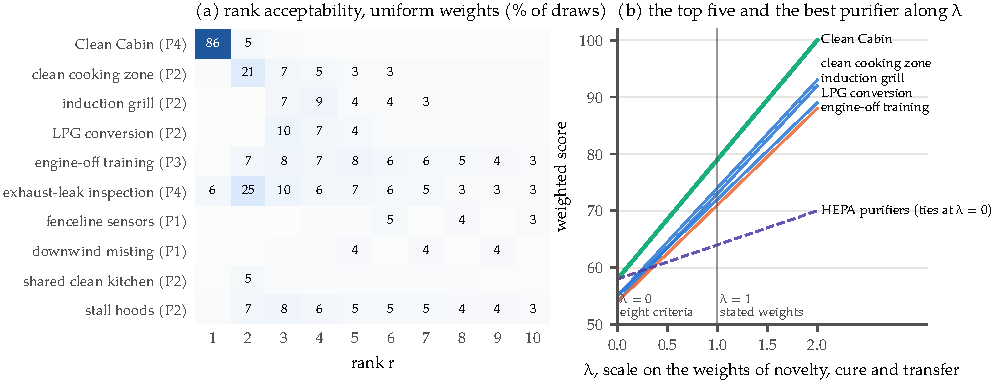
\includegraphics[width=\textwidth]{fig8-smaa}
\caption{(a) Rank acceptability of the ten leading rows under uniform weights, the share of 10,000 draws in which each row holds each rank. (b) Weighted score of the top five and of the best purifier as the weights of novelty, cure and transfer are scaled together by \(\lambda\).}\label{fig:smaa}\end{figure}

\section{Step 5: failure-mode analysis fixes the design specification}\label{sec:premortem}
The leading design on the school-gate block after scoring, gate orchestration (arrival slots and engine-off staging for buses, a just-in-time call for cars, a rolling lane, a dashboard, a gate sensor, 79 of 90), was subjected to a premortem \citep{Klein2007}: assume it has been piloted and has failed, and explain why, a method that rests on the prospective-hindsight finding of \citet{Mitchell1989}. To make the output examinable it was structured as a failure modes and effects analysis \citep{IEC60812}: modes enumerated layer by layer (heat, traffic mechanics, behaviour, institutions, the instrument, the mechanism, the market, the course), each given a severity from a definition fixed in advance (\emph{fatal}, the design as specified does not deliver its claim, \emph{major}, a large part of the effect or the pilot is lost, \emph{minor}, friction), and each tied to a graph edge or a fetched source. Twenty-nine modes, 5 fatal, 18 major, 6 minor (Figure~\ref{fig:premortem}). Four of the fatal modes are mechanisms rather than execution risks (Table~\ref{tab:fatal}), and the fifth is that an app releasing children on a parent's position handles minors' location data, which a school is unlikely to sign with a student group as data controller within a term. Two more cut the design's claims: the car half exists as a product, PickupLine \citep{iSchoolRide}, and the classroom carry-over measured in a naturally ventilated UK classroom \citep{Kumar2020} and in Barcelona \citep{Rivas2014} would be much smaller in a sealed, air-conditioned room if the indoor-to-outdoor ratios of 0.2 to 0.6 measured in Kuwait homes \citep{Yuan2020} transfer. Scored with the modes in, gate orchestration is 57.

\begin{table}[t]\centering\small
\caption{The four fatal mechanisms of a gate-side design, and the design rule each one sets.}\label{tab:fatal}
\begin{tabular}{@{}lp{7.6cm}p{5.6cm}@{}}\toprule
mode & mechanism and evidence & rule for the design\\ \midrule
F1 heat & in Abu Dhabi the idle is the air conditioning: a bus staged engine-off in September has no cooling, and the idle-reduction evidence \citep{AFDC2015} is a cold-climate cab-comfort document & never ask anyone to sit in the heat with the engine off\\
F2 relocation & a just-in-time call moves the wait, drivers and nannies already arrive early and wait around the school \citep{E247pickup}, the idling moves to the next street & remove the emission, not the place it happens\\
F5 the morning & the call exists only at dismissal, the morning is a throughput queue against a fixed bell and the threefold peak of \citet{Kumar2020} was a drop-off peak & act on both sessions of the day\\
F19 instrument & the gate increment is 3 to 4\,\ugm\ \citep{AdamsRequia2017,Ryan2013}, background explained 80.9\,\% of the variance at a New York dismissal \citep{RichmondBryant2009}, the Abu Dhabi background is 44\,\ugm\ and dust-dominated \citep{HEI2022uae}, low-cost optical sensors need site calibration and respond to humidity and composition \citep{Zheng2018} and do not see ultrafines & measure inside a closed volume, paired with the air outside the same bus, before and after\\
\bottomrule\end{tabular}\end{table}

\begin{figure}[t]\centering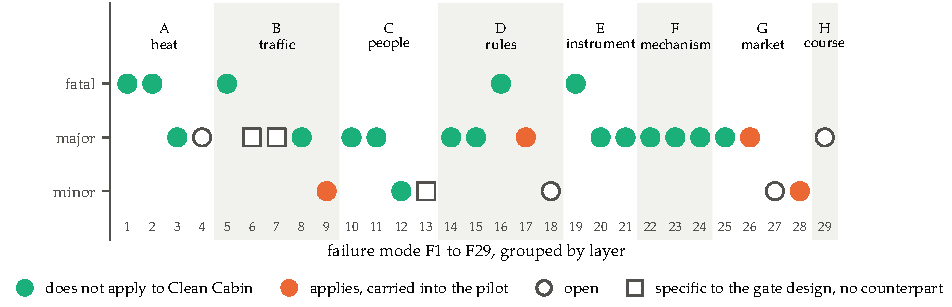
\includegraphics[width=0.95\textwidth]{fig9-premortem}
\caption{The 29 failure modes of a gate-side design by layer and severity, and whether each applies to Clean Cabin. None of the fatal modes does. Four apply and are carried into the pilot: the operator's consent, the buyer, restart pulses and the size of the team.}\label{fig:premortem}\end{figure}

\textbf{The specification.} The largest exposure term in the school system is the bus cabin, \num{4.11} of the commute block's \num{4.47}\,\load, six times the gate, and in-cabin concentrations are largely the bus's own doing, highest when idling with no other diesel vehicle in front \citep{Behrentz2005}. With the rules of Table~\ref{tab:fatal} the specification reads: act on the block's largest load term, at the source, inside a closed volume where the effect is measurable within one bus before and after, without engine-off in the heat, and without any parent, driver or app in the loop. Clean Cabin is that specification. On the unchanged rubric the row as inventoried scores 79, the top row alone (Figure~\ref{fig:pickscores}). The pilot scope in Section~\ref{sec:cabin} is narrower than that row, and re-scoring the narrowed design independently is listed in Section~\ref{sec:limits}. Of the 29 modes, 18 do not apply to it, four apply and are designed into the pilot (F9 restart pulses, F17 one operator's consent, F26 the buyer, F28 a three-student team), three concern the gate lane, bus slots and marshals and have no counterpart, and four are open (F4 dust days, F18 procurement and liability, F27 defensibility, F29 the instructor's question).

\section{Clean Cabin: find the buses that pollute their own cabin, fix why, verify}\label{sec:cabin}

\begin{figure}[t]\centering
\resizebox{\textwidth}{!}{\begin{tikzpicture}[x=1cm,y=1cm, font=\scriptsize]
% bus body
\draw[line width=0.7pt, ink2, rounded corners=4pt] (0,0) rectangle (8,2.3);
\foreach \x in {0.9,2.0,3.1,4.2,5.3} {\draw[ink2, line width=0.4pt, fill=grid] (\x,1.2) rectangle (\x+0.85,2.0);}
\draw[ink2, line width=0.5pt] (6.6,0) rectangle (7.4,2.0); \node[ink2] at (7.0,0.45) {door};
\foreach \x in {1.4,6.4} {\draw[ink2, fill=white, line width=0.6pt] (\x,0) circle (0.38);}
\draw[ink2, line width=0.4pt] (0,1.0) -- (0.6,1.0) -- (0.6,0.4) -- (0,0.4); \node[ink2, text width=1.6cm, align=center] at (-1.1,0.7) {engine bay: leak sealing, closed-crankcase kit};
% sensors
\draw[fill=b3, draw=b3] (3.8,2.3) rectangle (4.1,2.55); \node[above=1pt, b3] at (3.95,2.55) {roof sensor \(C_{\mathrm{roof}}\)};
\draw[fill=b3, draw=b3] (3.8,0.55) rectangle (4.1,0.8); \node[b3, anchor=east] at (3.7,0.67) {cabin sensor \(C_{\mathrm{cabin}}\)};
% tailpipe
\draw[line width=1pt, b2, -{Stealth[length=5pt]}] (0.2,0.15) -- (-0.3,0.15) -- (-0.3,2.9) -- (-0.7,3.3);
\node[b2, align=left, anchor=west] at (-0.6,3.55) {tailpipe routed up and to the off side,\\ away from the door and the cabin intake};
% state logger
\node[draw=b4, rounded corners=2pt, b4, align=center, text width=3.1cm, inner sep=2pt] at (6.6,3.2) {state log: idle or moving, HVAC fresh or recirculating, doors, load, T, RH, CO\(_2\)};
\draw[b4, line width=0.4pt] (6.6,2.72) -- (6.6,2.3);
% per-bus report
\node[draw=ink2, rounded corners=3pt, fill=white, align=center, inner sep=3pt, font=\scriptsize\bfseries] at (5.5,0.6) {report and cabin\\air grade per bus};
% formula
\node[anchor=west, align=left, font=\small] at (8.6,2.0) {\(R=\dfrac{C_{\mathrm{cabin}}}{C_{\mathrm{roof}}},\quad \Delta=C_{\mathrm{cabin}}-C_{\mathrm{roof}}\)};
\node[anchor=west, align=left, text width=5.2cm] at (8.6,0.8) {\(R\) and \(\Delta\) at idle, doors closed, HVAC recirculating, are the screening signal. The absolute cabin level is the exposure. The same three numbers on the same bus are the verification};
% timeline
\begin{scope}[shift={(0,-1.55)}, x=0.95cm]
\node[anchor=west, font=\scriptsize\bfseries] at (0,0.42) {pilot, one term};
\foreach \w in {1,...,12} {\node[ink2] at (\w-0.5,-0.55) {\w};}
\node[ink2, anchor=east] at (0,-0.55) {week};
\draw[fill=b3, draw=none] (0,0.0) rectangle (3,0.28); \node[white] at (1.5,0.14) {diagnose, validate};
\draw[fill=b1, draw=none] (3,0.0) rectangle (7,0.28); \node[white] at (5,0.14) {classify the source, repair};
\draw[fill=b4, draw=none] (7,0.0) rectangle (12,0.28); \node[white] at (9.5,0.14) {re-log, verify, report and grade per bus};
\node[anchor=north west, ink2, text width=15.2cm, align=left] at (0,-0.8) {Weeks 1 to 3: paired sensors on 10 to 20 buses, idling and moving, both sessions, with the state log, and a borrowed black-carbon or particle-number instrument beside the cheap sensors on 2 to 4 of them. Success, fixed in advance: for every flagged bus the idle cabin excess \(\Delta\) after the repair falls, within-bus and paired, into the range of the buses that were not flagged, and the source found is written down. Read-outs: \(R\), \(\Delta\) and the absolute cabin level before and after per bus, the source class, the repair done, its cost and consumables.};
\end{scope}
\end{tikzpicture}}
\caption{The service on one bus: two paired sensors, a state log, the source-side repairs that a diagnosis can call for, the per-bus report and grade, and the pilot.}\label{fig:design}\end{figure}

\textbf{What is built.} Clean Cabin 1.0 is diagnose, identify the source, repair, verify. It is not a retrofit kit: the evidence below shows that school buses can pollute their own cabin and that source-side repairs remove most of it, and the service exists to find which buses in Abu Dhabi do, why, and whether the repair worked. \emph{Diagnose} (Figure~\ref{fig:design}): two low-cost PM and CO\(_2\) sensors per bus, one in the cabin and one on the roof, co-located and cross-calibrated before installation, logging at idle and in motion together with the state of the bus, idling or moving, HVAC on fresh air or recirculating, doors, passenger load, route, cabin temperature and humidity. Three numbers are read per state: the cabin level \(C_{\mathrm{cabin}}\), the excess \(\Delta=C_{\mathrm{cabin}}-C_{\mathrm{roof}}\) and the ratio \(R\). The ratio is a screening signal, not a proof. An indoor-to-outdoor ratio depends on the HVAC mode, the air exchange rate, the speed, the filter and on what the passengers stir up, so a sealed bus on a dusty day can read \(R<1\) with its own exhaust inside, and a clean bus on a clean day can read \(R>1\) on a few micrograms. A bus is flagged on the excess at idle with doors closed and the HVAC recirculating, the state in which outside air enters least and the bus's own emissions show most \citep{Behrentz2005}, read against the fleet's spread, and the absolute cabin level is reported as the exposure in its own right. Low-cost optical sensors do not see the ultrafine fraction that diesel exhaust is rich in, drift with humidity and composition and need site calibration \citep{Zheng2018}, so a borrowed black-carbon or particle-number instrument runs beside them on 2 to 4 buses for the validation, and the matched pair on each bus cancels what the two cheap sensors share. \emph{Identify the source.} Before any hardware, the make, model year, engine, fuel, crankcase configuration, after-treatment and maintenance history of every bus in the pilot are recorded. The retrofit evidence below is from US buses of model years 1991 to 2006 with open crankcase ventilation, the population the EPA verifications cover \citep{EPASpiracle}. A modern engine with closed crankcase ventilation and after-treatment has no such fix to receive, and on such a fleet the diagnosis is what remains. A flagged bus is classified: an exhaust leak, an open-crankcase engine, HVAC infiltration through the intake, seals or filter, a high roadside background, a tailpipe geometry that recirculates into the door or intake, or no identifiable source. \emph{Repair.} The smallest compatible fix for the class found. For a leak, seal it. For an open-crankcase engine, a compatible closed-crankcase filtration system, which carries a coalescing element replaced at every oil change or 500 hours, or 1,000 hours with an indicator \citep{EPASpiracle}, so it is a consumable and is costed as one. For infiltration, inspect and replace the intake seals and filter. For a roadside background, a recirculation and filtration setting. For a recirculating tailpipe, a correction only as an OEM or operator-approved modification, since exhaust routing carries backpressure, heat, warranty and vehicle-approval consequences. For no identifiable source, no engine work at all. Ordinary maintenance repairs come first in the pilot. \emph{Verify.} The same three numbers on the same bus after the repair, a paired within-bus comparison. \emph{Report and grade.} Each bus receives a diagnostic report with its numbers, its source class, the repair and its cost, the operator receives the fleet's distribution, and each bus receives a cabin-air grade set from its verified numbers, the idle excess after the repair against the fleet's range. The grade is the incentive: an operator whose buses carry it has something to show a school, a school has something to write into a transport contract and check, and a parent has something to ask for. In the pilot the grade goes to the school and the operator on paper. It goes onto the bus, in public, once the local validation has shown that the numbers repeat across days, routes and HVAC settings, because a single noisy reading turned into a letter would mislead. The climate-aware idle timer of the inventoried row is out of the pilot as well: in Abu Dhabi the cabin is hot for most of the school year, so a timer keyed to cabin temperature idles most of the time, and its benefit is unmeasured. It is a later test.

\begin{figure}[t]\centering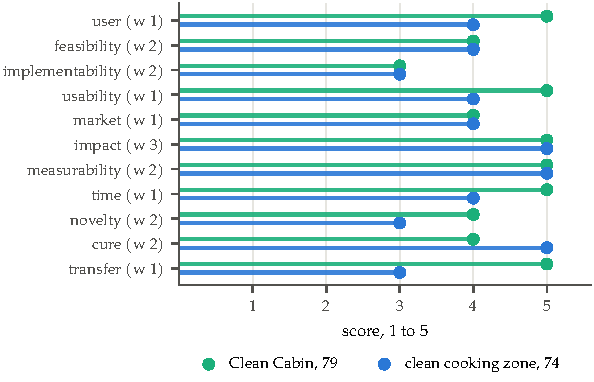
\includegraphics[width=0.6\textwidth]{fig11-pickscores}
\caption{The eleven criterion scores of the Clean Cabin row as inventoried against the runner-up. It leads or ties on nine criteria and trails only on cure, where replacing a fuel removes the emission outright. The pilot scope of this section is narrower than the row.}\label{fig:pickscores}\end{figure}

\textbf{Mechanism and prior art} (Figure~\ref{fig:priorart}). Dual-tracer measurements on two Seattle buses in 2005 attribute, with windows closed, 13.4 of 26\,\ugm\ of in-cabin PM\(_{2.5}\) to the bus's own emissions, 12 of that 13.4 from the crankcase, and with windows open 1.7 of 12 \citep{DualTracer2011}. The share is about half in the closed state, a seventh in the open one, and it is two buses. The ride is a tenth of a child's day and a third of its black carbon exposure \citep{Behrentz2005}, with in-bus black carbon of 0.9 to 19\,\ugm\ and NO\(_2\) of 64 to 220\,\ugm\ \citep{Sabin2005}. The kit is proven in the cabin: on a test track a closed-crankcase system cut in-cabin ultrafine counts by 50 to over 100\,\%, a tailpipe filter without it did not, and a well-maintained inspected bus ran 2.7\,\ugm\ in the cabin \citep{Rowan2008}. On route, crankcase filters with an oxidation catalyst cut in-cabin hopanes, PAH and aliphatics by 37, 50 and 43\,\% \citep{Pueblo2009}, tests in three states, as cited by \citet{EPARebate2023}, found 50 to 60\,\% lower cabin particles, and across 188 buses cleaner fuel or retrofits ran 10 to 50\,\% lower on board with respiratory outcomes to match \citep{Adar2015}. One study found no unequivocal cabin decrease despite tailpipe cuts of 20 to 94\,\% \citep{EST2011}, which is why every bus is diagnosed before and after. Outcomes follow: 2,656 retrofitted Georgia buses raised respiratory fitness and English scores \citep{Austin2019}, and a randomised rebate programme raised attendance \citep{EPARebate2023}. Every prior instance was a government retrofit or rebate programme delivered fleet-wide, and one of them found no unequivocal cabin decrease despite the tailpipe cut, which is the case for diagnosing before fixing. A per-bus diagnosis and verification sold as a service, a source classification per bus, and any measurement of a school-bus cabin in the UAE: none was found. The novelty score of the inventoried row also counted a cabin-temperature timer, deferred here. The evidence being twenty years old is what lets the pilot promise a measured result within the term.

\begin{figure}[t]\centering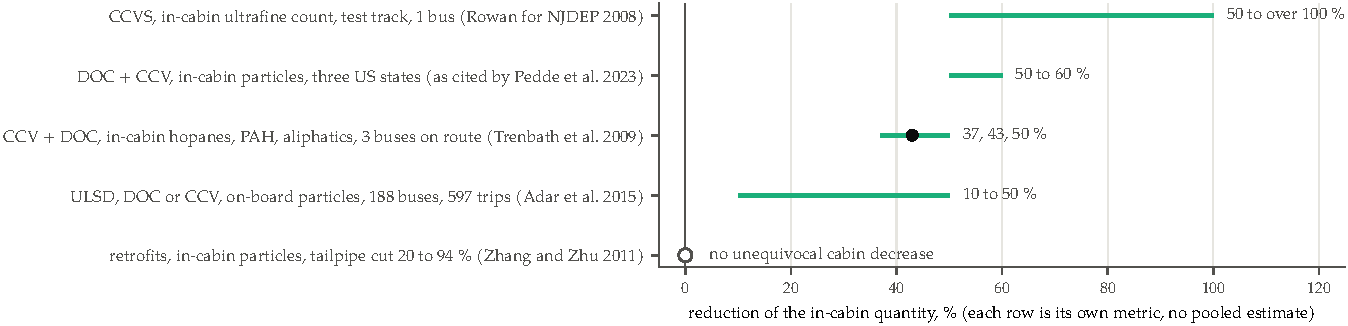
\includegraphics[width=0.95\textwidth]{fig10-priorart}
\caption{Measured in-cabin reductions from the source-side kit, one row per study with its own metric and sample. No pooled estimate is drawn because the quantities differ.}\label{fig:priorart}\end{figure}

\textbf{Scale and market.} 237,111 children on 8,568 buses run by 206 operators for 672 schools and nurseries in 2024 \citep{ADM2024buses}, and for the 2026 to 2027 year more than 10,000 licensed buses expected to carry more than 279,000 pupils \citep{GN2026buses}, 18\,\% more than the count the load arithmetic of Section~\ref{sec:load} uses. That is 80 minutes a day at 13\,\ugm\ above ambient if the transported increment holds here, and a regulator whose transport policy, as reported, fixes journey length, supervision and who may collect a child \citep{KT2025adek} and says nothing reported about the air in the cabin. Who pays is an assumption until asked: the likely buyer is a school writing a verifiable clause into its transport contract or an operator answering one, not the individual parent, and the first work of the pilot is to interview three schools and two operators before a sensor is bought. Diagnosis, report and grade are sold per bus, repairs go through the operator's workshop, the re-check is termly and renews the grade, and the regulator can adopt the grade as a standard later without the pilot needing it. The first partner is the university's own shuttle service, to be confirmed, then one operator's twenty buses at one school. If the fleet turns out to be modern and most buses clean, the finding is the product: which buses carry the excess, and why.

\section{What is assumed, transported or unmeasured}\label{sec:limits}
Every increment in Table~\ref{tab:load} is transported from another city and no UAE measurement exists for any of them: the literature says school buses elsewhere add about 13\,\ugm\ to a child's ride, and the pilot tests whether Abu Dhabi's do, it does not assume it. The near-road load rests on an unsourced fraction of residents within 300 m of an arterial, which a GIS overlay would settle. Time at the gate, the delivery shift and the car commute are stated assumptions, and the 8-hour day is the statutory figure. The load ignores susceptibility \citep{Gauderman2004,Gauderman2007} and toxicity per microgram, and a child weight of two or three does not change the ranking. Leakage is size-blind, modularity has a resolution parameter, the weights are ordinal readings of the literature and not an interaction matrix, and the partition depends on which studies were read (Table~\ref{tab:dropout}), which is why the decomposition is reported as a menu of candidates with its stability and not as a theorem about controllability. The eleven scores were assigned by the authors against written anchors and no inter-rater reliability was measured. The score-jitter analysis of Section~\ref{sec:funnel} bounds what that could cost (rank 1 in 48\,\% rather than 86\,\%), and the next step is an independent scoring of the narrowed design by each author and one outsider, with the agreement reported. The cabin-to-roof ratio is a screening signal whose reading depends on the HVAC state and the passengers, and the cheap sensors do not see ultrafines, both of which the pilot design answers with the state log, the excess, the absolute level and the reference instrument. Whether any Abu Dhabi bus has an open crankcase, and therefore whether the best-evidenced repair applies at all, is unknown until the fleet inventory is taken. The failure-mode list is what three people enumerated in a session, and the seven modes marked open or not applicable were classified, not analysed. The fuel and CO\(_2\) of idling for cooling are outside the design, and so, for now, is the idle timer.

\section{Conclusion}
A cited graph, decomposed by a network method inspired by near-decomposability, turns a system into a menu of four candidate problems and measures how stable the menu is under re-weighting and under missing evidence. An exposure load with every input sourced ranks it. Morphological generation on the graph's edges produces 332 interventions that can be enumerated rather than remembered. A gated, weighted, stochastically stress-tested rubric ranks them, and a failure-mode analysis fixes the specification the winner has to meet. The result is not a retrofit kit for school buses. It is a measurement-driven service for the more than 279,000 children who ride them in Abu Dhabi: find which buses pollute their own cabin, identify why, apply the smallest compatible source-side repair, and verify that it worked, on evidence twenty years old that we found nowhere applied here, holding rank 1 in 86\,\% of rankings drawn with no information about our weights and leading, without dominating, when our own scores are shaken. The next step is one operator's twenty buses, a paired sensor in each, and the fleet's engine list.

\appendix
\section{Reproducibility}\label{app:repro}
\begin{sloppypar}Two folders hold everything. \texttt{agrl130-graph/}: \texttt{nodes.csv}, eight \texttt{edges-lane*.csv} with matching \texttt{sources-lane*.md}, \texttt{decompose.py} (build, leakage, Louvain, resolution sweep, Leiden and greedy cross-checks, sensitivity, the problem node sets of Figure~\ref{fig:coverage}), \texttt{perturb.py} (the 200 weight trials per block), \texttt{dropout.py} (Table~\ref{tab:dropout}), \texttt{lanes/anchor\_test.py}. \texttt{agrl130-solutions/}: \texttt{inventory.py} (332 interventions with edge, class, gates and scores), \texttt{extra.py} (novelty, cure, transfer), \texttt{build.py} (writes \texttt{solutions.csv} and the workbook), \texttt{robustness.py} (SMAA over the weights, leave-one-out, the \(\lambda\) sweep), \texttt{scorejitter.py} (SMAA over the scores). \texttt{agrl130-report/figures.py} draws every figure from those files, \texttt{refs.py} resolved every reference at Crossref and \texttt{bib.py} wrote the bibliography from the returned records.\end{sloppypar}

\bibliographystyle{plainnat}
\bibliography{refs}
\end{document}
